\documentclass[english]{article}
\usepackage[T1]{fontenc}
\usepackage[latin9]{inputenc}
\usepackage{babel}
\usepackage{graphicx}
\usepackage{subfigure}
\usepackage{float}
\setlength{\parindent}{0pt}
\usepackage{amsmath}


\begin{document}

\title{Lab 3: Lens \& Lighting\\ -------------------------------- \\ \Large Sensors and Digitization}
\author{ \ Armine Vardazaryan, Songyou Peng \\ arminevardazaryan@gmail.com, psy920710@gmail.com}
\date{5rd December 2015}

\maketitle

\section{Introduction}
This lab offers us a chance to have a insight of lens and light.
In the first part, we will choose different lens and extension rings, and then talk about the influence on the acquisition.
The second part is mainly about the observation of some objects under different light source, and do defect detection. 

\section{Lens}
At the very beginning of this lab, we want to compute the "Spatial Resolution". In the Figure \ref{fig:one}, we try to demonstrate the length of this fork by putting a ruler next to it.
We can see the length of the fork is about 214 $mm$ and the number of pixels between this length is $(1310 - 40) = 1270$, so we can easily get the spatial resolution as below:
$$
resolution = \frac{number of pixels}{length} = \frac{214}{1270} = 0.1685\ mm/pixel
$$
\begin{figure}[H]
	\centering
	
\includegraphics[width=1\linewidth]{Pictures/spatial_resolution.png}
	\caption{Picture for computing spatial resolution}
	\label{fig:one}
\end{figure} 

Now we will compute the focal length of the lens to test whether we use a correct lens or not.
In order to get Figure \ref{fig:one}, our intial working distance is 500$mm$.
And we know our CCD height and width are 6.6$mm$ and 8.8$mm$ respectively.
So after applying the formula:
\begin{align*} 
	Focal\ length\ of\ the\ height &= \frac{working\ distance * CCD\ height}{Object\ height + CCD\ height}\\
	&= \frac{500 \times 6.6}{214 + 6.6} \\
	&= 15.00mm
\end{align*}
It turns out we use correct lens because the 16$mm$ length is the closest lens that we have to 15mm.
\section{Extension Rings}
In this part, we try various lens and rings in order to observe the influence of extension ring.
We know that extension ring will get the lens further away from the focal plane, which leads to the decrease of working distance.
So with an extension ring, you can take a closer picture of your object and include more information and more part of the object.\\
\\
First, we try 50$mm$ lens with 5$mm$ ring, image shown in Figure \ref{fig:twoa}.
At this time, working distance that we measure is 300$mm$.
When we remove the ring, the image is Figure \ref{fig:twob} and working distance now is 515$mm$. Obviously, more information and bigger fork we get in the Figure \ref{fig:twoa}.
\begin{figure}[H]
	\centering
	\subfigure[Object with 5$mm$ ring]{\label{fig:twoa}
	
\includegraphics[width=0.45\linewidth]{Pictures/ring_50.png}
	}
	\subfigure[Object without ring]{\label{fig:twob}
	
\includegraphics[width=0.45\linewidth]{Pictures/without_ring_50.png}
	}
	\caption{Object with 50$mm$ lens}
	\label{fig:two}
\end{figure}

In another example we use 35$mm$ lens and compare coin images by using different extension rings, which is shown in Figure \ref{fig:three}.
It is easy to be noticed that the image with 20$mm$ ring contains more information than the one with 5$mm$ ring.\\
\\
So, if you want to put the object full of your image, choosing a proper extension ring would be helpful.
\begin{figure}[H]
	\centering
	\subfigure[Object with 5$mm$ ring]{\label{fig:threea}
	
\includegraphics[width=0.45\linewidth]{Pictures/bonus/coin35+5.png}
	}
	\subfigure[Object with 20$mm$ ring]{\label{fig:threeb}
	
\includegraphics[width=0.45\linewidth]{Pictures/bonus/35+20_coin.png}
	}
	\caption{Object with 35$mm$ lens}
	\label{fig:three}
\end{figure}

\section{Lighting}
\subsection{Silhouette Analysis}
In this section the goal was to use a lighting system to capture the contours of an object and to detect defects on a shiny surface.
In order to observe the contours of an object, we introduced a background lighting.
As a background lighting we used a fiber optic light pad. 
The fork was placed onto the light pad, and because of the hight intensity of the light, the contours of the fork were sharply visible as shown in Figure \ref{fig:four}.\\
\begin{figure}[H]
	\centering
	{\label{fig:}
	
\includegraphics[width=0.5\linewidth]		{Pictures/contour/untitled.png}
	}
	\caption{Fork contours captured with 16$mm$ lens}
	\label{fig:four}
\end{figure}
To make the edged even more pronounced, we used the Measurement \& Automation Explorer software to apply  filters onto the captured image. We used inverse, inverse binary and inverse log filters with the results as shown in Figure \ref{fig:five}.\\
\begin{figure}[H]
	\centering
	\subfigure[Inverse filter]{\label{fig:inv}
	
\includegraphics[width=0.45\linewidth]{Pictures/contour/inv.png}
	}
	\subfigure[Inverse binary filter]{\label{fig:invbin}
	
\includegraphics[width=0.45\linewidth]{Pictures/contour/invbin.png}
	}
		\subfigure[Inverse log filter]{\label{fig:invlog}
	
\includegraphics[width=0.45\linewidth]{Pictures/contour/invlog.png}
	}
	\caption{Applying filters on the image of a fork}
	\label{fig:five}
\end{figure}
\subsection{Defect Detection on a Shiny Surface}
In this part, we tried detecting surface defects,
such as scratches, on a shiny surface (the fork).
This time, in order to observe the surface, we changed the lighting to illuminate the part being examined.
We used a circular fiber optic light source to do that.
Since we are only interested in the surface of the fork, we used a 5mm extension ring to decrease the field of view of the camera.
\begin{figure}[H]
	\centering
	\subfigure[Original image of surface]{\label{fig:orig_surf}
	
\includegraphics[width=0.5\linewidth]{Pictures/scr/16+5.png}
	}
		\subfigure[Surface with an inverse filter]{\label{fig:invlog}
	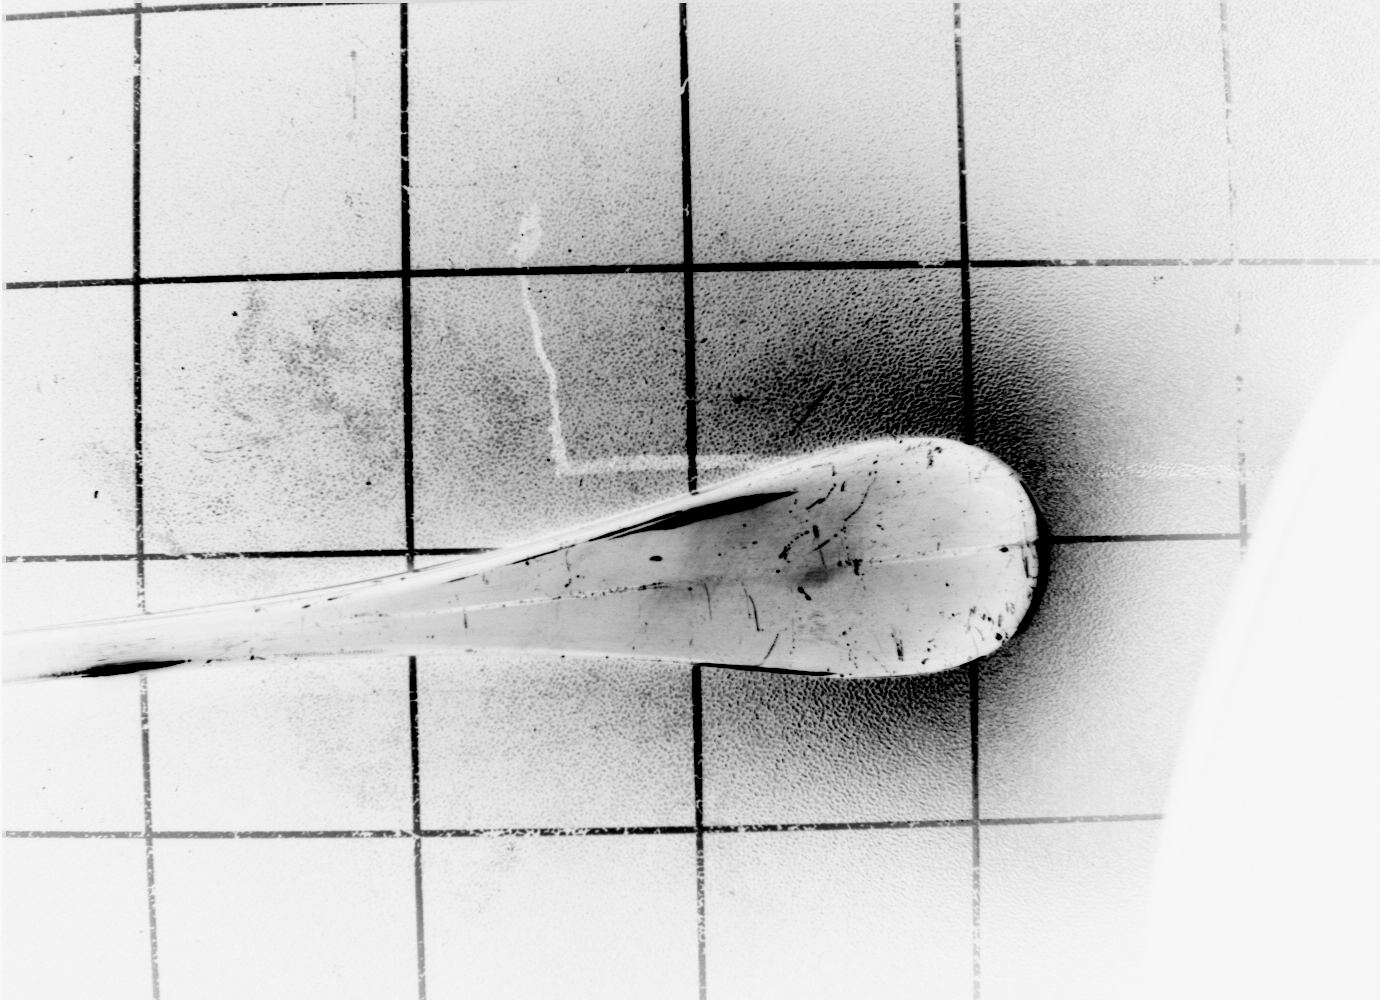
\includegraphics[width=0.5\linewidth]{Pictures/scr/inv16+5.png}
	}
	\caption{Surface defect detection with a 16mm lens + 5mm ext. ring}
	\label{fig:six}
\end{figure}
In Fig. \ref{fig:six} we see the scratches on the polished surface of the fork clearly.
However, to make the defects more visible we applied an inverse filter on the same image.
\section{Surface Inspection}
In this part of the experiment we tried to pick the best systems to capture the following three objects: an oil filter, a magnet and a coin.
For all of the images taken in this part we used an LED light source provided with the system.
First, we took an image of the center of an oil filter using a 35mm lens (Figure \ref{fig:seven}).
\ref{fig:four}.\\
\begin{figure}[H]
	\centering
	{\label{fig:}
	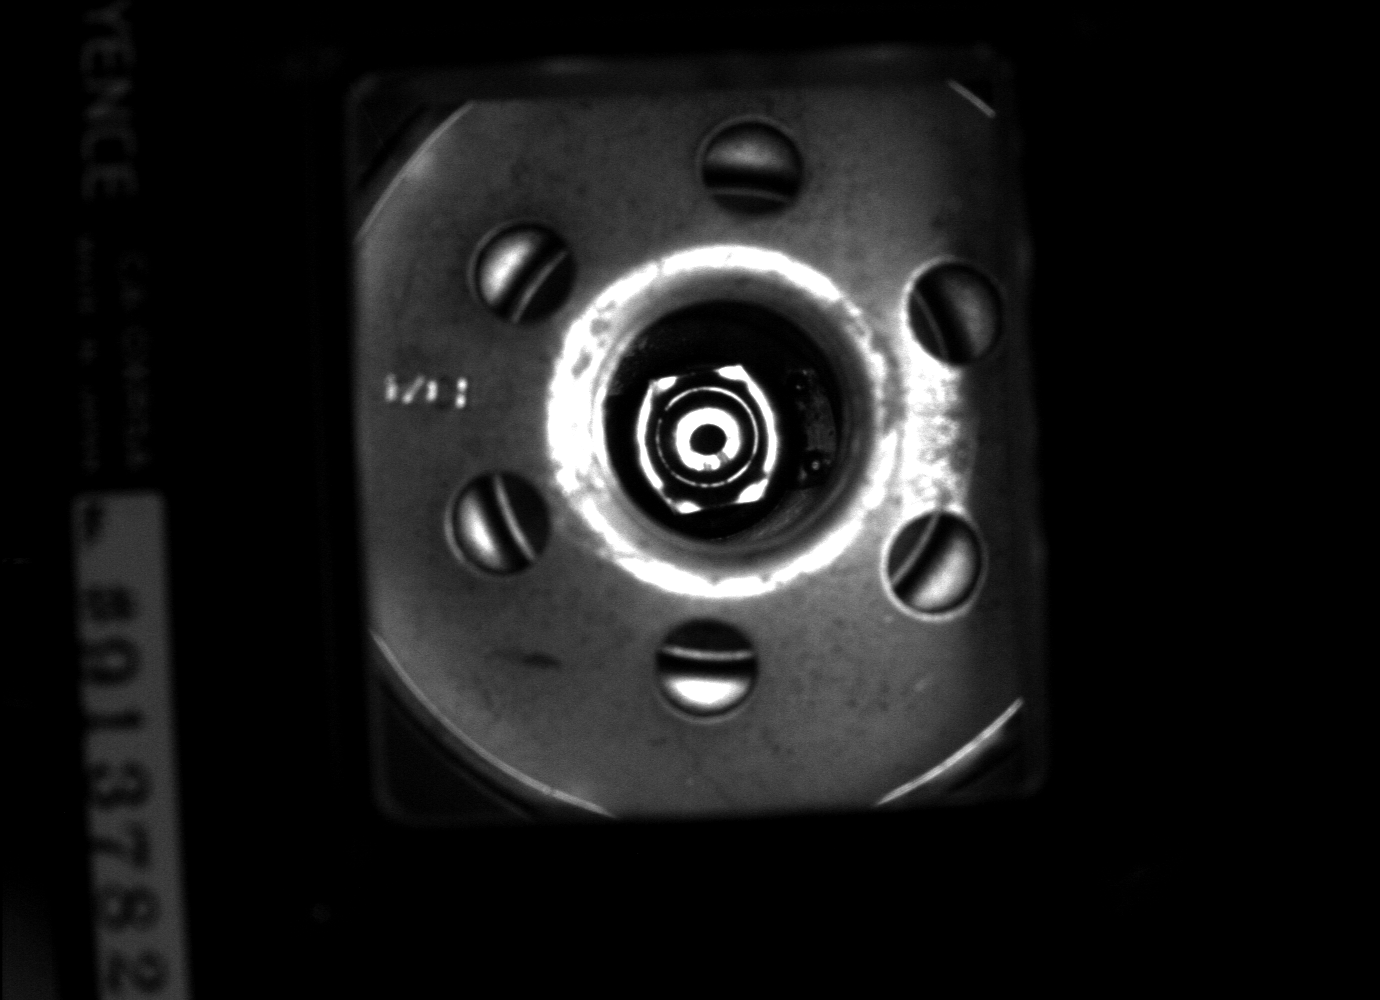
\includegraphics[width=0.6\linewidth]		{Pictures/bonus/oil_filter_adj.png}
	}
	\caption{Oil Filter image take with a 35mm lens}
	\label{fig:seven}
\end{figure}
To estimate the price of this kind of a lens, we chose a similar product:\\
\begin{itemize}
\item 35mm Dia. x 70mm FL Uncoated, Double-Convex Lens - \$42.00\\
\end{itemize}
Then, we tried to pick a system of a lens and an extension tube to focus well on the surface of a small magnet.
We chose a 35mm lens and a 5mm extension ring, which permits to see the pattern on the surface and scratches very clearly.
And because we used an extension ring, the working distance was reduced to less than 10cm. 
A smaller working distance, in turn, decreased the field of view greatly.
\begin{figure}[H]
	\centering
	{\label{fig:}
	
\includegraphics[width=0.7\linewidth]		{Pictures/bonus/35+5.png}
	}
	\caption{Image of a magnet taken with a 35mm lens + 5mm ext. tube}
	\label{fig:eight}
\end{figure}
To estimate the price of this imaging system we went on www.edmundoptics.com, to choose an appropriate system. In reality we would need a light source, a camera, a frame grubber, etc., but here we are only taking into account the lens and the extension ring, as the rest of the system is reused.\\
\begin{itemize}
\item 
5mm Length, C-Mount Extension Tube - \$22.50\\
\item 35mm Dia. x 70mm FL Uncoated, Double-Convex Lens - \$42.00
\end{itemize}
Which amounts to \$64.50. 
And lastly, we adjusted the system to focus on the surface of a penny (Fig. \ref{fig:nine}).
\begin{figure}[H]
	\centering
	{\label{fig:}
	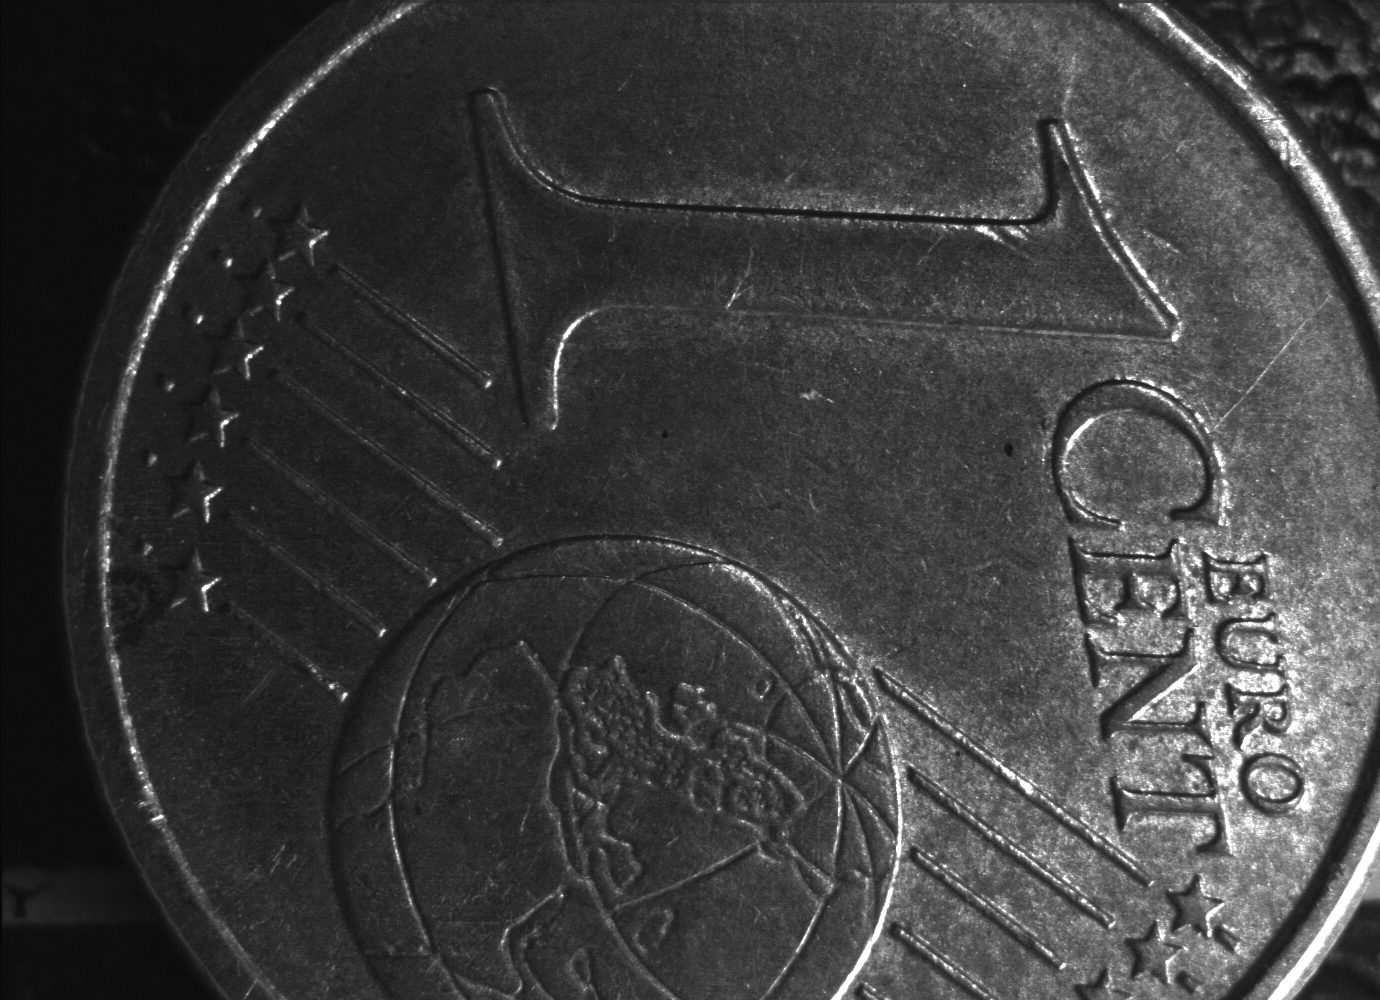
\includegraphics[width=0.7\linewidth]		{Pictures/bonus/50+20coin_distance_20mm_adj.png}
	}
	\caption{Image of a penny taken with a 50mm lens + 20mm ext. tube}
	\label{fig:nine}
\end{figure}
We chose the following system of a lens and an extension tube for this image:\\
\begin{itemize}
\item 50 x 44mm FL Condenser Lens, \$32.50\\
\item 2 x 10mm Length, C-Mount Extension Tube, \$45.00\\
\end{itemize}
This system amount to a total of \$77.50.

\section{Conclusion}
In conclusion, in this lab we studied the working principle behind lenses, lighing and extension tubes.
We experimented with different types of lenses and extension rings, and used the system to detect defects of a surface of an object. In addition, we estimated the pricing of different optical systems using an online source.

\section{References}
{[}1{]} - https://photographylife.com/what-is-an-extension-tube\\
{[}2{]} - http://www.edmundoptics.com
\end{document}